\section*{Problem 3: Neural Nets: Written Questions [30 pts]}
\label{sec:written}

\textbf{Note:} We strongly encourage you to do the written part of this homework before the programming, as it will help you gain familiarity with the calculations you will have to code up in the programming section. We suggest that for each of these problems, you write out the equation required to calculate each value in terms of the variables we created ($a_j, z_j, b_k$, etc.) before you calculate the numerical value.

\textbf{Note:} For all questions which require numerical answers, round up your final answers to four decimal places. For integers, you may drop trailing zeros. We will use column vectors for the data and neural network layers, be consistent with the question in your answers involving vectors. If your answer involves application of an operator element-wise to a vector or a matrix, state it explicitly.

 \begin{figure}[h]
        \centering
        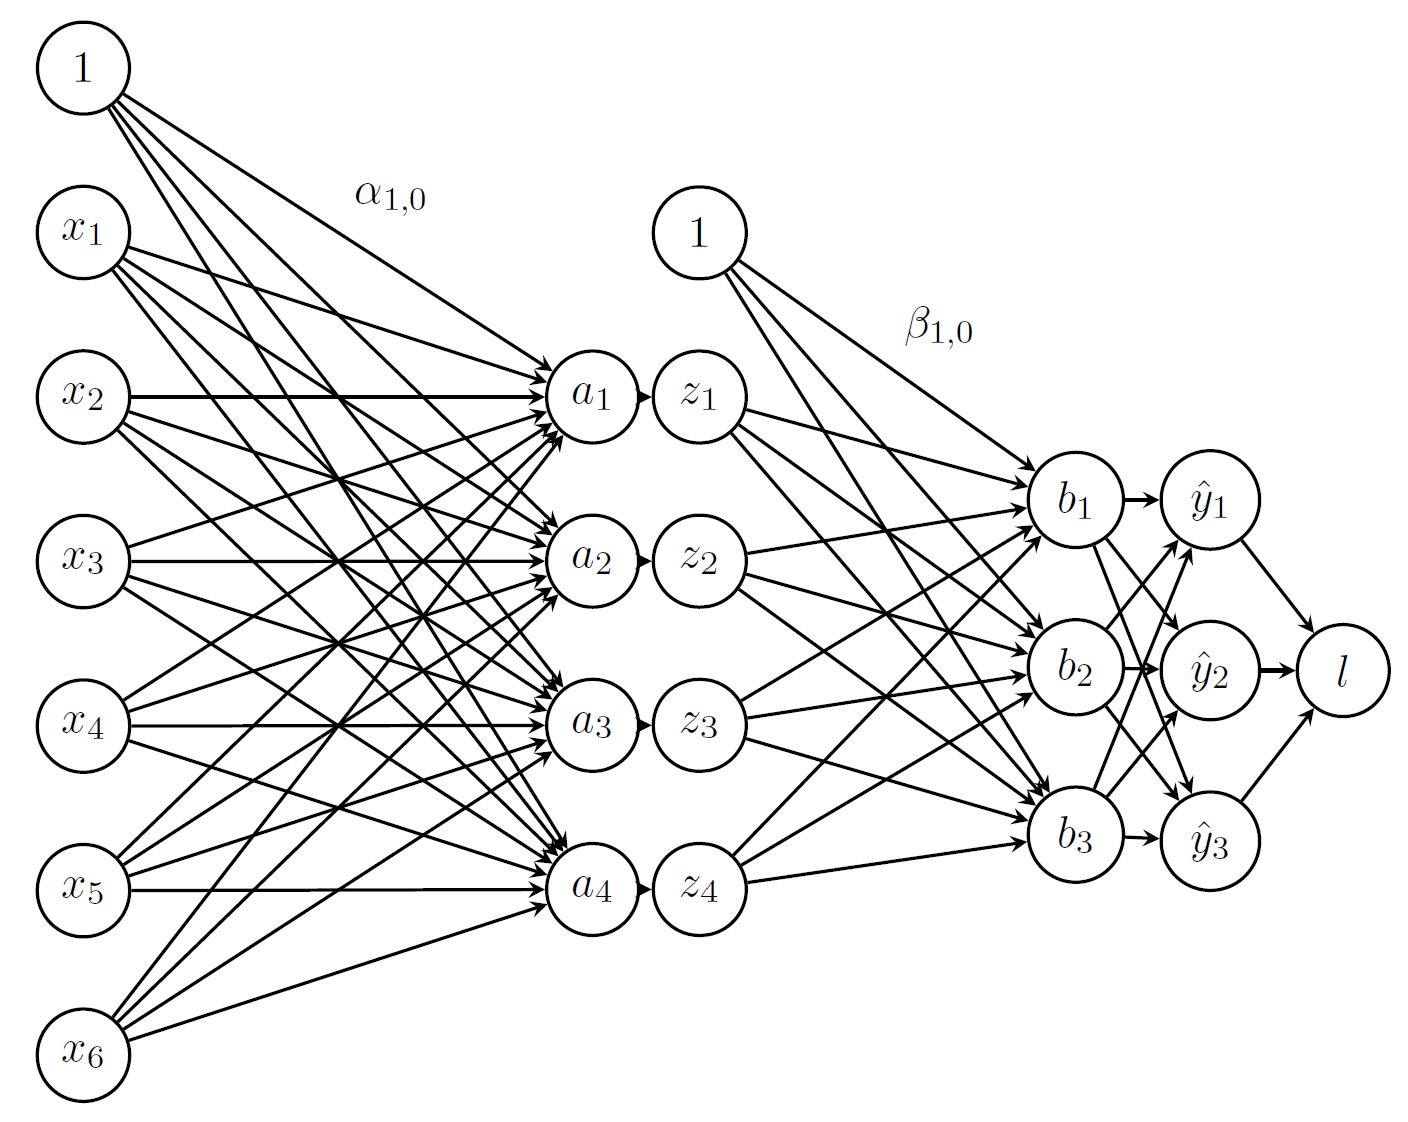
\includegraphics[height=9cm]{img/network.png}
        \caption{A One Hidden Layer Neural Network}
        \label{fig:oneHL}
    \end{figure}

\subsubsection*{\textcolor{purple}{Network Overview}}
Consider the neural network with one hidden layer shown in Figure \ref{fig:oneHL}. The input layer consists of 6 features $\xv = [x_1,...,x_6]^T$, the hidden layer has 4  nodes $\zv = [z_1,...,z_4]^T$, and the output layer is $\hat{\yv} = [\hat{y}_1, \hat{y}_2, \hat{y}_3]^T$ that sums to one over 3 classes. We also add a bias to the input, $x_0 = 1$ and the hidden layer $z_0 = 1$, both of which are fixed to $1$.


We adopt the following notation:
\begin{enumerate}
    \item Let \textcolor{magenta}{$\boldsymbol{\alpha}$} be the matrix of weights from the inputs to the hidden layer.
    \item Let \textcolor{magenta}{$\boldsymbol{\beta}$} be the matrix of weights from the hidden layer to the output layer.
    \item Let \textcolor{magenta}{$\alpha_{j,i}$} represent the weight going \textit{to} the node $z_j$ in the hidden layer \textit{from} the node $x_i$ in the input layer (e.g. $\alpha_{1,2}$ is the weight from $x_2$ to $z_1$)
    \item Let \textcolor{magenta}{$\boldsymbol{\beta}_{k,j}$} represent the weight going \textit{to} the node $y_k$ in the output layer \textit{from} the node $z_j$ in the hidden layer.
    \item We will use a \emph{sigmoid activation function (\textcolor{magenta}{$\sigma$})} for the hidden layer and a \emph{softmax} for the output layer. 
\end{enumerate}

\subsubsection*{\textcolor{purple}{Network Details}}
Equivalently, we define each of the following. 

The input:
\begin{align}
\xv=[x_1,x_2,x_3,x_4,x_5,x_6]^T
\end{align}

Linear combination at first (hidden) layer:
\begin{equation}
a_j= \alpha_{j,0} + \sum_{i=1}^6 \alpha_{j,i}x_i,\quad j \in \{1,\ldots,4\}
\end{equation}

Activation at first (hidden) layer:
\begin{align}
z_j &= \sigma(a_j) = \frac{1}{1+\exp(-a_j)},\quad  j \in \{1,\ldots,4\}
\end{align}

Linear combination at second (output) layer:
\begin{equation}
b_k = \beta_{k,0} + \sum_{j=1}^4 \beta_{k,j}z_j,\quad  k \in \{1,\ldots,3\}
\end{equation}

Activation at second (output) layer:
\begin{equation}
\hat{y}_k = \frac{\exp(b_k)}{\sum\limits_{l=1}^3 \exp(b_l)},\quad  k \in \{1,\ldots,3\}
\end{equation}

Note that the linear combination equations can be written equivalently as the product of the weight matrix with the input vector. We can even fold in the bias term $\alpha_0$ by thinking of $x_0 = 1$, and fold in $\beta_0$ by thinking of $z_0 = 1$.

\subsubsection*{\textcolor{purple}{Loss}}

We will use cross entropy loss, $\ell(\hat{\yv},\yv)$. If $\yv$ represents our target (true) output, which will be a \textcolor{purple}{one-hot vector} representing the correct class, and $\hat{\yv}$ represents the output of the network, the loss is calculated as (note that the $\log$ terms are in base $e$):
\begin{equation}
   \ell(\hat{\yv},\yv) = - \sum_{k=1}^3 y_k \log(\hat{y}_k)
\end{equation}
%%%%%%%%%%%%%%%%%%%%

\begin{enumerate}
\item \textbf{[6 pts]} In the following questions you will derive the matrix and vector forms of the previous equations which define our neural network. These are what you should hope to program in order to avoid excessive loops and large run times.\\
When working these out it is important to keep a note of the vector and matrix dimensions in order for you to easily identify what is and isn't a valid multiplication. Suppose you are given a training example: $\xv^{(1)}=[x_1,x_2,x_3,x_4,x_5,x_6]^T$ with \textbf{label class 2}, so $\yv^{(1)}=[0,1,0]^T$. We initialize the network weights as:
\begin{center}
$$\boldsymbol{\alpha^*}=
    \begin{bmatrix}
    \alpha_{1,1} & \alpha_{1,2} & \alpha_{1,3} & \alpha_{1,4} & \alpha_{1,5} & \alpha_{1,6} \\
    \alpha_{2,1} & \alpha_{2,2} & \alpha_{2,3} & \alpha_{2,4} & \alpha_{2,5} & \alpha_{2,6} \\
    \alpha_{3,1} & \alpha_{3,2} & \alpha_{3,3} & \alpha_{3,4} & \alpha_{3,5} & \alpha_{3,6} \\
    \alpha_{4,1} & \alpha_{4,2} & \alpha_{4,3} & \alpha_{4,4} & \alpha_{4,5} & \alpha_{4,6}
    \end{bmatrix}$$
    
$$\boldsymbol{\beta^*}=
    \begin{bmatrix}
    \beta_{1,1} & \beta_{1,2} & \beta_{1,3} & \beta_{1,4} \\
    \beta_{2,1} & \beta_{2,2} & \beta_{2,3} & \beta_{2,4} \\
    \beta_{3,1} & \beta_{3,2} & \beta_{3,3} & \beta_{3,4}
    \end{bmatrix}
$$
\end{center}
    
We want to also consider the bias term and the weights on the bias terms (${\alpha}_{j,0}$ and ${\beta}_{k,0})$. To account for these we can add a new column to the beginning of our initial weight matrices. 

$$\boldsymbol{\alpha}=
    \begin{bmatrix}
    \textcolor{blue}{\alpha_{1,0}} & \alpha_{1,1} & \alpha_{1,2} & \alpha_{1,3} & \alpha_{1,4} & \alpha_{1,5} & \alpha_{1,6} \\
    \textcolor{blue}{\alpha_{2,0}} & \alpha_{2,1} & \alpha_{2,2} & \alpha_{2,3} & \alpha_{2,4} & \alpha_{2,5} & \alpha_{2,6} \\
    \textcolor{blue}{\alpha_{3,0}} & \alpha_{3,1} & \alpha_{3,2} & \alpha_{3,3} & \alpha_{3,4} & \alpha_{3,5} & \alpha_{3,6} \\
    \textcolor{blue}{\alpha_{4,0}} & \alpha_{4,1} & \alpha_{4,2} & \alpha_{4,0} & \alpha_{4,4} & \alpha_{4,5} & \alpha_{4,6}
    \end{bmatrix}$$
    
$$\boldsymbol{\beta}=
    \begin{bmatrix}
    \textcolor{blue}{\beta_{1,0}} & \beta_{1,1} & \beta_{1,2} & \beta_{1,3} & \beta_{1,4} \\
    \textcolor{blue}{\beta_{2,0}} & \beta_{2,1} & \beta_{2,2} & \beta_{2,3} & \beta_{2,4} \\
    \textcolor{blue}{\beta_{3,0}} & \beta_{3,1} & \beta_{3,2} & \beta_{3,3} & \beta_{3,4}
    \end{bmatrix}$$

    And we can set our first value of our input vectors to always be 1 ($x_0^{(i)} = 1$), so our input becomes: $$\xv^{(1)}=[\textcolor{blue}{1},x_1,x_2,x_3,x_4,x_5,x_6]^T$$
    
    
    \begin{enumerate}
        \item \textbf{[1 pt]} By examining the shapes of the initial weight matrices, how many neurons (or nodes) do we have in the first hidden layer of the neural network? (Not including the bias neuron)
        
        \begin{tcolorbox}[fit,height=1cm, width=2cm, blank, borderline={1pt}{-2pt}]
            %solution 
        \end{tcolorbox}

        
        
        
        \item \textbf{[1 pt]} How many output neurons will our neural network have?
        
        \begin{tcolorbox}[fit,height=1cm, width=2cm, blank, borderline={1pt}{-2pt}]
            %solution 
        \end{tcolorbox}

        
        
        
        
        \item \textbf{[1 pt]} What is the vector $\av$ whose elements are made up of the entries $a_j$ in equation (4). Write your answer in terms of $\alphav$ and $\xv^{(1)}$.
        
        
        \begin{tcolorbox}[fit,height=1cm, width=4cm, blank, borderline={1pt}{-2pt}]
            %solution 
        \end{tcolorbox}
        
        
        
        
        \item \textbf{[1 pt]} What is the vector $\zv$ whose elements are made up of the entries $z_j$ in equation (5)? Write your answer in terms of $\av$.
        
        \begin{tcolorbox}[fit,height=2cm, width=14cm, blank, borderline={1pt}{-2pt}]
            %solution 
        \end{tcolorbox}

        
        \item \textbf{[1 pt]} \textbf{Select one:} We cannot take the matrix multiplication of our weights $\betav$ and our vector $\zv$ since they are not compatible shapes. Which of the following would allow us to take the matrix multiplication of $\betav$ and $\zv$ such that the entries of the vector $\bv = \betav\zv$ are equivalent to the values of $b_k$ in equation (5)? 
        
        \begin{list}{}
        \item $\circle$ Remove the last column of $\betav$
        \item $\circle$ Remove the first row of $\zv$
        \item $\circle$ Append a value of 1 to be the first entry of $\zv$
        \item $\circle$ Append an additional column of 1's to be the first column of $\betav$ 
        \item $\circle$ Append a row of 1's to be the first row of $\betav$ 
        \item $\circle$ Take the transpose of $\betav$
        \end{list}
        
        
        
        \item \textbf{[1 pt]} What are the entries of the output vector $\hat{\yv}$? Your answer should be written in terms of $b_1,b_2,b_3$.
        
        \begin{tcolorbox}[fit,height=3.3cm, width=14cm, blank, borderline={1pt}{-2pt}]
            %solution 
        \end{tcolorbox}
        
        
    \end{enumerate} 

\item \textbf{[7 pts]} We will now derive the matrix and vector forms for the backpropagation algorithm.

$$\frac{d\ell}{d\alphav} = 
    \begin{bmatrix}
        \adj{\alpha_{10}} & \adj{\alpha_{11}} & \dots  & \adj{\alpha_{1M}} \\
        \adj{\alpha_{20}} & \adj{\alpha_{21}} & \dots  & \adj{\alpha_{2M}} \\
        \vdots      & \vdots      & \ddots & \vdots \\
        \adj{\alpha_{D0}} & \adj{\alpha_{D1}} & \dots  & \adj{\alpha_{DM}}
    \end{bmatrix}$$




The mathematics which you have to derive in this section jump significantly in difficultly, you should always be examining the shape of the matrices and vectors and making sure that you are comparing your matrix elements with calculations of individual derivatives to make sure they match (e.g. the element of the matrix $(\frac{d\ell}{d\alpha})_{2,1}$ should be equal to $\frac{d\ell}{d\alpha_{2,1}}$  ). Recall that $\ell$ is our loss function defined in equation (1.8)
    
    \begin{enumerate}
        \item \textbf{[1 pt]} The derivative of the softmax function with respect to $b_k$ is as follows:
        $$\frac{d\hat{y}_l}{db_k} = \hat{y}_l(\Ib[k=l]-\hat{y}_k)$$ 
        where $\Ib[k=l]$ is an indicator function such that if $k=l$ then it it returns value 1 and 0 otherwise. 
        Using this, write the derivative $\frac{d\ell}{db_k}$ in a smart way such that you do not need this indicator function. Write your solutions in terms of $\hat{y}_k,y_k$.
        
        
        \begin{tcolorbox}[fit,height=2cm, width=12cm, blank, borderline={1pt}{-2pt}]
            %solution 
        \end{tcolorbox}
        
        
        \item \textbf{[1 pt]} What are the elements of the vector $\frac{d\ell}{db}$? (Recall that  $\yv^{(1)}=[0,1,0]^T$)
        
        
        \begin{tcolorbox}[fit,height=1cm, width=6cm, blank, borderline={1pt}{-2pt}]
            %solution 
        \end{tcolorbox}
        
        
        
        \item \textbf{[1 pt]} What is the derivative $\frac{d\ell}{d\beta}$? Your answer should be in terms of $\frac{d\ell}{d\bv}$ and $\zv$.
        
        
        \begin{tcolorbox}[fit,height=3cm, width=12cm, blank, borderline={1pt}{-2pt}]
            %solution 
        \end{tcolorbox}
        
        
        
        \item \textbf{[1 pt]} Explain in one short sentance why must we go back to using the matrix $\betav^*$ (The matrix $\betav$ without the first column of ones) when calculating the matrix $\frac{d\ell}{d\alpha}$?
        
        
        \begin{tcolorbox}[fit,height=1cm, width=15cm, blank, borderline={1pt}{-2pt}]
            %solution 
        \end{tcolorbox}
        
        
        
        \item \textbf{[1 pt]} What is the derivative $\frac{d\ell}{d\zv}$? Your answer should be in terms of $\frac{d\ell}{d\bv}$ and $\betav^*$
        
        
        \begin{tcolorbox}[fit,height=3cm, width=12cm, blank, borderline={1pt}{-2pt}]
            %solution 
        \end{tcolorbox}
        
        
        \item \textbf{[1 pt]} What is the derivative $\frac{d\ell}{d\av}$ in terms of $\frac{d\ell}{d\zv}$ and $\zv$?
        
        
        \begin{tcolorbox}[fit,height=3cm, width=12cm, blank, borderline={1pt}{-2pt}]
            %solution 
        \end{tcolorbox}
        
        
        \item \textbf{[1 pt]} What is the matrix $\frac{d\ell}{d\alpha}$? Your answer should be in terms of $\frac{d\ell}{d\av}$ and $x^{(1)}$.
        
        
        \begin{tcolorbox}[fit,height=3cm, width=12cm, blank, borderline={1pt}{-2pt}]
            %solution 
        \end{tcolorbox}

\end{enumerate}



%%%%%%%%%%%%%%%%%%%%%%%%
\newpage
\subsubsection*{\textcolor{purple}{Prediction}}
When doing prediction, we will predict the \textcolor{purple}{$\argmax$} of the output layer. For example, if $\hat{\yv}$ is such that $\hat{y}_1=0.3,~ \hat{y}_2=0.2,~ \hat{y}_3=0.5$ we would predict class 3 for the input $\xv$. If the true class from the training data $\xv$ was $2$ we would have a \textcolor{purple}{one-hot vector} $\yv$ with values $y_1=0$,~ $y_2=1$,~ $y_3=0$.
    
\item \textcolor{black}{\textbf{[8 pts]}}
     We initialize the weights as:
\begin{center}
$$\boldsymbol{\alpha^*}=
    \begin{bmatrix}
    2 & 1 & -1 & -1 & 0 & -2 \\
    0 & 1 & 0 & -1 & 1 & 3 \\
    -1 & 2 & 1 & 3 & 1 & -1 \\
    1 & 3 & 4 & 2 & -1 & 2
    \end{bmatrix}$$
$$\boldsymbol{\beta^*}=
    \begin{bmatrix}
    2 & -2 & 2 & 1 \\
    3 & -1 & 1 & 2 \\
    0 & -1 & 0 & 1
    \end{bmatrix}
$$
\end{center}
    
And weights on the bias terms (${\alpha}_{j,0}$ and ${\beta}_{j,0})$ are initialized to 1.
    
    You are given a training example $\xv^{(1)}=[1,0,1,0,1,0]^T$ with label class 2, so $\yv^{(1)}=[0,1,0]^T$. Using the initial weights, run the feed forward of the network over this training example (without rounding during the calculation) and then answer the following questions. 
    %In your responses, round to four decimal places---if the answer is an integer you need not include trailing zeros. 
    
    \begin{enumerate}
        \item \textbf{[1 pt]} What is the value of $a_1$?
        
        \begin{tcolorbox}[fit,height=1cm, width=2cm, blank, borderline={1pt}{-2pt}]
            %solution 
        \end{tcolorbox}
        
        \item \textbf{[1 pt]} What is the value of $z_1$?
        
        \begin{tcolorbox}[fit,height=1cm, width=2cm, blank, borderline={1pt}{-2pt}]
         %solution 
        \end{tcolorbox}
        
        \item \textbf{[1 pt]} What is the value of $a_3$?
        
        \begin{tcolorbox}[fit,height=1cm, width=2cm, blank, borderline={1pt}{-2pt}]
        %solution 
        \end{tcolorbox}
        
        \item \textbf{[1 pt]} What is the value of $z_3$?
        
        \begin{tcolorbox}[fit,height=1cm, width=2cm, blank, borderline={1pt}{-2pt}]
            %solution 
        \end{tcolorbox}
        
        \item \textbf{[1 pt]} What is the value of $b_2$?
        
        \begin{tcolorbox}[fit,height=1cm, width=2cm, blank, borderline={1pt}{-2pt}]
            %solution 
        \end{tcolorbox}
        
        \item \textbf{[1 pt]} What is the value of $\hat{y}_2$?
        
        \begin{tcolorbox}[fit,height=1cm, width=2cm, blank, borderline={1pt}{-2pt}]
            %solution 
        \end{tcolorbox}
        
        \item \textbf{[1 pt]} Which class value we would predict on this training example?
        
        \begin{tcolorbox}[fit,height=1cm, width=2cm, blank, borderline={1pt}{-2pt}]
            %solution 
        \end{tcolorbox}

        \item \textbf{[1 pt]} What is the value of the total loss on this training example?
        
        \begin{tcolorbox}[fit,height=1cm, width=2cm, blank, borderline={1pt}{-2pt}]
            %solution 
        \end{tcolorbox}
        
    \end{enumerate}
    
  %  \clearpage
\item \textcolor{black}{\textbf{[4 pts]}} Now use the results of the previous question to run backpropagation over the network and update the weights. Use the learning rate $\eta=1$. 
    
    Do your backpropagation calculations without any rounding then answer the following questions: (in your final responses round to four decimal places)
    
     \begin{enumerate}
        \item \textbf{[1 pt]} What is the updated value of ${\beta}_{2,1}$?
        
        \begin{tcolorbox}[fit,height=1cm, width=2cm, blank, borderline={1pt}{-2pt}]
            %solution 
        \end{tcolorbox}
        
        \item \textbf{[1 pt]} What is the updated weight of the hidden layer bias term applied to $y_1$ (i.e. ${\beta}_{1,0}$)?
        
        \begin{tcolorbox}[fit,height=1cm, width=2cm, blank, borderline={1pt}{-2pt}]
            %solution 
        \end{tcolorbox}
        
        \item \textbf{[1 pt]} What is the updated value of ${\alpha}_{3,4}$?
        
        \begin{tcolorbox}[fit,height=1cm, width=2cm, blank, borderline={1pt}{-2pt}]
            %solution 
        \end{tcolorbox}
        
        \item \textbf{[1 pt]} If we ran backpropagation on this example for a large number of iterations and then ran feed forward over the same example again, which class would we predict?
        
        \begin{tcolorbox}[fit,height=1cm, width=2cm, blank, borderline={1pt}{-2pt}]
            %solution 
        \end{tcolorbox}
        
    \end{enumerate}

\clearpage
\item \textcolor{black}{\textbf{[5 pts]}} Let us now regularize the weights in our neural network. For this question, we will incorporate L2 regularization into our loss function $\ell(\hat{\yv},\yv)$, with the parameter $\lambda$ controlling the weight given to the regularization term. 
\begin{enumerate}
    \item \textbf{[1 pt]} Write the expression for the regularized loss function of our network after adding L2 regularization (\textbf{Hint:} Remember that bias terms should not be regularized!) 
    \begin{tcolorbox}[fit,height=3cm, width=15cm, blank, borderline={1pt}{-2pt}]
            %solution 
    \end{tcolorbox}
        
    \item \textbf{[1 pts]} Compute the regularized loss for training example $\xv^{(1)}$ (assume $\lambda$ = 0.01 and use the weights before backpropagation)
    \begin{tcolorbox}[fit,height=1cm, width=2cm, blank, borderline={1pt}{-2pt}]
            %solution 
    \end{tcolorbox}
    
     \item \textbf{[1 pts]} For a network which uses the regularized loss function, write the gradient update equation for $\alpha_{j,i}$ . You may use $\frac{\partial \ell(\hat{\yv},\yv)}{\partial \alpha_{j,i}}$ to denote the gradient update w.r.t non-regularized loss and $\eta$ to denote the learning rate.
    \begin{tcolorbox}[fit,height=3cm, width=15cm, blank, borderline={1pt}{-2pt}]
            %solution 
    \end{tcolorbox}
    
    
    \item \textbf{[2 pts]} Based on your observations from previous questions, \textbf{select all statements which are true}:
    \begin{list}{}
    \item $\square$ The non-regularized loss is always higher than the regularized loss 
    \item $\square$ As weights become larger, the regularized loss increases faster than non-regularized loss
    \item $\square$ On adding regularization to the loss function, gradient updates for the network become larger
    \item $\square$ When using large initial weights, weight values decrease more rapidly for a network which uses regularized loss 
    \item $\square$ None of the above
    \end{list}
    
\end{enumerate}
\end{enumerate}